% TODO: add in the referee tag for the submission
%\documentclass[global,twocolumn,referee]{svjour}
\documentclass[global,twocolumn]{svjour}
\usepackage{cite}
\usepackage{amsmath}
% \usepackage{amsthm}
\usepackage{amsfonts}
\usepackage{url}
\usepackage{comment}
\usepackage{paralist}
\usepackage{graphicx}
\graphicspath{{./figs/}}
\usepackage{listings}
\usepackage[usenames,dvipsnames,svgnames,table]{xcolor}
\usepackage{flushend}
\usepackage{hyperref}
\usepackage[firstpage]{draftwatermark}
\usepackage[lighttt]{lmodern}
\usepackage[normalem]{ulem}

\definecolor{dkgreen}{rgb}{0,0.6,0}
\definecolor{mauve}{rgb}{0.58,0,0.82}
\definecolor{light-gray}{gray}{0.88}

\lstdefinestyle{myML}
{frame=none,
  basicstyle=\ttfamily,
  language=ML,
  aboveskip=3mm,
  belowskip=3mm,
  showstringspaces=false,
  columns=flexible,
  numbers=none,
  numberstyle=\tiny\color{gray},
  commentstyle=\color{dkgreen},
  stringstyle=\color{mauve},
  breaklines=false,
  breakatwhitespace=true,
  tabsize=2,
  linewidth=2\linewidth
}

\lstdefinestyle{agree}
{frame=none,
  basicstyle=\ttfamily,
  language=ML,
  aboveskip=3mm,
  belowskip=3mm,
  showstringspaces=false,
  columns=flexible,
  numbers=none,
  numberstyle=\tiny\color{gray},
  commentstyle=\color{dkgreen},
  stringstyle=\color{mauve},
  breaklines=false,
  breakatwhitespace=true,
  tabsize=2,
  linewidth=2\linewidth,
  morecomment=[l]{--},
  escapeinside={*}{*},
  morekeywords={eq, bool, guarantee, assume, true, false, pre, not, and, or, property, const, Historically, Since, Once, event, annex, Implementation, process, subcomponents}
}

\hyphenation{op-tical net-works semi-conduc-tor Cake-ML}

\newcommand{\konst}[1]{\ensuremath{\mathsf{#1}}}
\newcommand{\imp}{\Rightarrow}
\newcommand{\set}[1]{\ensuremath{\{ {#1} \}}}
\newcommand{\sem}[1]{\ensuremath{[\![ #1 ]\!]}}
\newcommand{\kstar}[1]{\ensuremath{{#1}^{*}}}
\newcommand{\Lang}[1]{\ensuremath{{\mathcal L}({#1})}}
\newcommand{\Eqs}{\ensuremath{\mathit{Eqs}}}
\newcommand{\itelse}[3]{\mbox{$\mathtt{if}\ {#1}\ \mathtt{then}\ {#2}\ \mathtt{else}\ {#3}$}}

\newcommand{\figref}[1]{Fig.~\ref{#1}}
\newcommand{\secref}[1]{Sec.~\ref{#1}}
\newcommand{\lineref}[1]{Line~\ref{#1}}
\newcommand{\linesref}[2]{Lines~\ref{#1}--\ref{#2}}
% \newcommand{\eqref}[1]{Eq.~\ref{#1}}

% Latex trickery for infix div operator, from stackexchange

\makeatletter
\newcommand*{\bdiv}{%
  \nonscript\mskip-\medmuskip\mkern5mu%
  \mathbin{\operator@font div}\penalty900\mkern5mu%
  \nonscript\mskip-\medmuskip
}
\makeatother

\newcommand{\ie}{\textit{i.e.}}
\newcommand{\eg}{\textit{e.g.}}
\newcommand{\etal}{\textit{et al.}}
\newcommand{\etc}{\textit{etc.}}
\newcommand{\adhoc}{\textit{ad hoc}}

% \theoremstyle{plain}
% \newtheorem{theorem}{Theorem}
% \newtheorem{lemma}{Lemma}

% \theoremstyle{definition}
% \newtheorem{definition}{Definition}

% \theoremstyle{remark}
% \newtheorem{remark}{Remark}

\journalname{Software and Systems Modeling}

\newif\ifREVISIONS
\REVISIONSfalse

\begin{document}
\title{
  Synthesizing Verified Components for Cyber Assured Systems Engineering
  \thanks{DISTRIBUTION STATEMENT A.  Approved for public release.}
}

\author{
  Eric Mercer\inst{1}    \and
  Konrad Slind\inst{2}   \and
  Isaac Amundson\inst{2} \and
  Darren Cofer\inst{2}   \and
  Junaid Babar\inst{3}   \and
  David Hardin\inst{3}
}

\institute{
  Brigham Young University        \\
  Provo, Utah                     \and
  Applied Research and Technology \\
  Collins Aerospace               \\
  Minneapolis, Minnesota          \and
  Applied Research and Technology \\
  Collins Aerospace               \\
  Cedar Rapids, Iowa
}

\date{Received: date / Revised version: date}

\maketitle

\begin{abstract}
Cyber-physical systems, such as avionics, must be tolerant to
cyber-attacks in the same way they are tolerant to random faults: they
must gracefully recover, or safely shut down, as requirements dictate.
We have developed a workflow for creating, and inserting,
high-assurance components implementing cyber-resiliency into a
model-based systems engineering environment.  Example high-assurance
components are filters, which guard against malformed input, and
runtime monitors, which guard against spoofing and other malicious
behavior. A formal specification in the form of a \emph{code contract}
defines each high-assurance component and is developed with the
support of \emph{test contracts} for testing the specified behavior.
Once tested, model checking used to verify that the added
high-assurance component indeed addresses system-level cyber
requirements.  Implementations for these high-assurance components are
directly synthesized from their code contracts and are backed up by
proofs showing that high-level specifications map in a
semantics-preserving way to code generated by a verified compiler.  We
report on a case study that cyber-hardened a UAV system by inserting
high assurance components to harden the open source Air Force Research
Laboratory's OpenUxAS services for route planning.  The case study
demonstrates that synthesizing correct implementations from code
contracts is feasible in real-world systems engineering.

\end{abstract}

\section{Introduction} \label{sec:intro}

\egm{Add to introduction and related work, that what is done at
Galois called Copilot. Its a stream processing langague that generates
code from the specification. Copilot to C. Effectively CodeGen from
Lustre. Bounds how far needed to look in past for any value.}

In recent years, aerospace stakeholders have realized that avionics
systems are subject to possible cyber-attacks just like other
cyber-physical systems.
%
\footnote{This work was funded in part by the
Defense Advanced Research Projects Agency (DARPA).  The views
expressed are those of the authors and do not reflect the official
policy or position of DARPA or the U.S. Government.}
%
Thus, in addition to being fault-tolerant, safety-critical avionics
systems must also be {\em cyber-resilient}.  Cyber-resiliency means
that the system is tolerant to cyber-attacks just as safety-critical
systems are tolerant to random faults: they recover and continue to
execute their mission function, or safely shut down, as requirements
dictate.

Unfortunately, systems engineers are currently given few development
tools to help answer even basic questions about potential
vulnerabilities and ways to mitigate vulnerabilities.  They instead
rely on process-oriented checklists and guidelines.  Cyber
vulnerabilities are often discovered during penetration testing late
in the development process; or worse yet, they may be discovered only
after the product has been fielded, necessitating extremely expensive
and time-consuming remediation. This is not a sustainable development
model.

%% The DARPA Cyber Assured Systems Engineering (CASE) project is targeted
%% at developing tools for design, analysis, and verification that enable
%% systems engineers to {\em design-in} cyber-resiliency for complex
%% cyber-physical systems.

We have been developing the {\em BriefCASE} toolsuite to address this need.
\brfcs\ is a Model-Based Systems Engineering (MBSE) environment
built in the Open Source AADL\footnote{AADL is the acronym for
Architecture Analysis and Design Language~\cite{aadl}.}  Tool
Environment (OSATE) to add new design, analysis, and code generation
capabilities for building cyber-resilient systems.

In this paper we describe how \brfcs\ facilitates inserting,
specifying, testing, and synthesizing high assurance components into a
system to improve its cyber-resiliency.  The main organizing concept
is that of an architecture-to-architecture \emph{security-improving
transform}, achieved via the insertion of a new architectural
component aimed at mitigating a cyber-vulnerability.  We describe two
cyber-resiliency transformations in this paper: (1) the insertion of a
filter to prevent malformed data from a malicious actor being
propagated to downstream components, and (2) the insertion of a
runtime monitor to detect (and alert) unexpected behaviors arising
from untrusted components.

A code contract is a formal specification in the Assume Guarantee
Reasoning Environment (\agr) language.
\agr\ is a compositional reasoning verification engine that uses \emph{contracts} on components to specify input and output properties and then prove whether or not those properties hold when given a sub-component implementation \cite{agree2013}.
The code contract language is Turing complete allowing the designer to
specify arbitrarily complex behavior.  These contracts are unit tested
for correctness with \emph{test contracts}.  Test contracts define
test scenarios to be implemented by the code contract under test.
\agr\ proves whether or not that code contract implementation is correct, enabling the designer to iteratively test the component behavior inside the \brfcs\ environment.
Once the behavior of the code contract is verified, \agr\ proves that---due to the newly
included high-assurance components---the hardened system meets its
cyber-resiliency requirements.

Another novel aspect of our workthe approach discussed in this manuscript is
the synthesis of the code contracts for the high-assurance components
to \ckml, a verified compiler implementation for the functional
programming language ML \cite{cakeml}.  This manuscript describes in
detail the synthesis path from code contracts to \ckml\ code,
providing a formal framework in which to argue correctness. \ckml\
then provides a verified compilation path to several different target
binaries (and also proving that the meaning of the \ckml\ source code
is exactly preserved in the final binaries).  A key contribution here
is that the code contract semantics are defined in such a way that
the \agr\ verification results for the code contract hold for the
deployed component, \ie, the component will detect and prevent the
indicated cyber-vulnerabilities over all possible finite
inputs. Preliminary work has shown how to lift this result to infinite
input traces as these systems are inherently reactive and intended to
run forever~\cite{case-verified-filter}, \cite{cakeml-space-cost}.

The manuscript further details a case study applying these
transformations with \brfcs\ to an Unmanned Aerial Vehicle (UAV)
system that uses the Air Force Research Laboratory's OpenUxAS services
for route planning.  OpenUxAS, as an open source product, is
considered \emph{untrusted}.  The UAV system is thus transformed to be
resilient to malicious behavior that may arise in the untrusted
component.  Here the transforms add filters to guard against malformed
input and monitors to guard against malicious flight plans from
OpenUxAS. The case study system is complex and shows the viability of
the approach in potential full-scale industrial design.

\brfcs\ is open source and publicly available \cite{fmide} as are the examples and case study discussed in this manuscript \cite{repo, phase2, camkes, case}.
Our approach currently applies to common cyber-vulnerabilities, such
as overflow, lack of input validation, and supply-chain issues;
however, other cyber-vulnerabilities such as side-channel attacks and
denial of service are not yet dealt with in our work.  Here, we do not
report on the invention of a new type of high-assurance component in
terms of capability; instead, our contribution is in the automated
synthesis of security-improving components from formal specifications
and a means to show that the synthesis is correct.

We now give a summary of the contributions detailed in this
manuscript.
\begin{compactitem}
  \item The language and semantics of code contracts to specify the behavior of high assurance components.
  \item Test contracts as a stylized mechanism to unit test code contracts inside the \brfcs\ framework with \agr.
  \item A synthesis path from code contracts to \ckml\ with a formal framework to argue correctness.
  \item A formal argument that \agr\ verification of code contracts carry over to the resulting binaries from the \ckml\ compiler.
  \item A case study that used the implementation of the approach in \brfcs\ to add cyber-resiliency to a non-trivial UAV system.
\end{compactitem}
The rest of this manuscript is organized as follows.
\secref{sec:overview} is an overview of the \brfcs\ environment and key tools in that environment relative to the contributions of this work. The approach is illustrated by a simple example in
\secref{sec:example}. Essential background on \agr\ verification and specification are
presented in \secref{sec:agree}.
The language and semantics of code contracts are defined in \secref{sec:code-contracts}, and test contracts are defined in \secref{sec:testing}.
The synthesis pathway is covered in Section~\ref{sec:synthesis}.
\secref{sec:case-study} discusses the case study.
This is followed by related work in \secref{sec:related-work}.
The conclusions and future work are in \secref{sec:conclusion}.

\begin{comment}
  BriefCASE incorporates model-level cyber analysis tools (presently
  GearCASE~\cite{gearcase2020} and DCRYPPS~\cite{dcrypps2019}) which can
  examine AADL models for potential vulnerabilities and suggest
  cyber-security requirements to mitigate them.  A library of
  architectural transforms guides the system engineer through automated
  model transformations that modify the architecture to address these
  requirements, possibly inserting new high-assurance components into
  the system.  Implementations for the new components are synthesized
  from formal specifications using
  SPLAT~\cite{slind-hcss2020},~\cite{formal-filter-synth-langsec}
  (Semantic Properties for Language and Automata Theory).


  Formal
  verification that the transformed system model meets its requirements
  is accomplished via \agr~\cite{agree2013} (Assume Guarantee Reasoning
  Environment).
  %The AGREE analysis \emph{assumes} properties on the inputs of a given component of the system, and attempts to formally prove the conjectured \emph{guarantees} of the output.
  \agr\ is a {\em compositional assume-guarantee} style model checker
  for AADL models that attempts to prove properties about one layer of
  an architecture using properties allocated to its subcomponents.
  Cyber-resilient code implementing the verified model is then
  automatically generated using the High Assurance Modeling and Rapid
  Engineering for Embedded Systems (HAMR) toolkit~\cite{hamr}.  If
  desired, this code can be targeted to the formally verified seL4
  secure microkernel~\cite{sel4-2009}.
\end{comment}


\ifREVISIONS
\subsection{SOSYM Journal Details}
The due date is \textbf{March} $22^\mathrm{nd}$, \textbf{2022}.
Go to \url{https://mc.manuscriptcentral.com/sosym/}. Create a new account (if you don't have one), login and go to the "Author"-section, select the link "Start New Submission" under Author Dashboard and select "Special Section Paper" as the paper type, and choose "MODELS 2021 Special Issue". Also, make sure to mention the MODELS 2021 special issue in the cover letter.
\fi

\ifREVISIONS
\subsection{Revisions}
\begin{compactitem}
  \item Revise the end of the abstract regarding the case studies to be consistent with what ends up in this version of the paper.
  \item Revise the end of the introduction that discusses the case studies to be consistent with what ends up in this version of the paper.
  \item Fix the link to the motivating example to point to the new repository once it is created. Fix in the next section too.
  \item Add discussion on the limitation of the approach: what attacks can and cannot be covered, can valid messages be rejected, etc.
\end{compactitem}
\fi

\section{Illustrative example}
\label{sec:example}
Show a filter, monitor, and gate form Phase II and indicate each of their intended roles.

\section{Compositional reasoning}
\label{sec:agree}

\newcommand{\globally}{\ensuremath{\mathbf{G}}}
\newcommand{\historically}{\ensuremath{\mathbf{H}}}
\newcommand{\assumes}{\ensuremath{A}}
\newcommand{\guarantees}{\ensuremath{P}}
\newcommand{\dispatch}{\ensuremath{\mathit{dispatch}}}
\newcommand{\complete}{\ensuremath{\mathit{complete}}}
\newcommand{\same}[1]{\ensuremath{\mathit{same}(#1)}}
\newcommand{\inputs}{\ensuremath{I}}
\newcommand{\outputs}{\ensuremath{O}}
\newcommand{\system}{\ensuremath{S}}
\newcommand{\components}{\ensuremath{C}}
\newcommand{\component}{\ensuremath{c}}
\newcommand{\schedule}{\ensuremath{\phi}}
\newcommand{\valid}{\ensuremath{\mathit{valid}}}
\newcommand{\dpred}{\ensuremath{\delta^\phi}}
\newcommand{\dispred}{\ensuremath{\mathbb{D}^\phi}}
\newcommand{\compred}{\ensuremath{\mathbb{C}^\phi}}
\newcommand{\dispredp}{\ensuremath{\mathbb{D}^{\phi\prime}}}
\newcommand{\compredp}{\ensuremath{\mathbb{C}^{\phi\prime}}}

The AGREE specification language is based on stream concepts, and
operators, from the Lustre language \cite{10.1145/41625.41641}. Thus
the setting is synchronous dataflow where the inputs and outputs of
components are streams, and contracts express relationships between
input and output streams. When considering a system of components,
data flows through the components in dependency order, with inputs
being propagated to outputs through all contracts until they stabilize
(can't propagate further). Therefore, the subcomponent contracts, and
thus the top-level model, must be acyclic. (An apparent syntactic
cycle, where a component is linked back to itself, may be broken
temporally by inserting delay elements.)  Once the data propagation
has stabilized, the model proceeds to the next input data in the input
streams. The semantics do not model computation or communication
delay. The output of one contract is seen at the input of any
downstream contract in the same step of the input data stream.

From the system and component contracts, AGREE generates a set of
verification conditions to show that a system's component
implementation is correct~\cite{agree2013}.  The AGREE model checker
is then invoked to prove or disprove the verification
conditions. Contracts and verification conditions are expressed in
\emph{past-time linear temporal logic} (PLTL).\footnote{KLS: citation
needed.}  PLTL is a logic enhanced with temporal operators able to
reason about the truth values of formulas through time.  Its semantics
are defined relative to a point in time $i$ and a finite trace of
system states $\pi = s_0, s_1, \ldots, s_i$.

The two PLTL operators necessary for the AGREE generated verification
conditions are $\globally$ (globally) that looks forward in time along
the trace and $\historically$ (historically) that looks backward in
time along the trace.  These are defined as
\begin{eqnarray*}
 (\pi, i) \models \globally(f) & \iff & \forall j \ge i, (\pi, j) \models f \\
(\pi, i) \models \historically(f) & \iff & \forall 0 \le j \le i, (\pi, j) \models f
\end{eqnarray*}
The $\models$-operator is read as \emph{satisfies}.  A trace at a
moment in time satisfies $\globally(f)$ if and only if it satisfies
$f$ in the current and all future states of $\pi$.  $\globally(f)$ is
invariant from the current moment into the future and $\historically$ is
invariant from the beginning of the trace to the current moment.

A \emph{system} $\system = (\inputs, \outputs, \assumes,
\guarantees,C)$, where $\inputs$ is the input set, $\outputs$ is the
output set, $\assumes$ is the set of assumptions, $\guarantees$ is the
set of guarantees, and $C$ are subcomponents.  A subcomponent
$\component$ is, hierarchically, also a system, and may be designated
by its own tuple $(\inputs_\component, \outputs_\component,
\assumes_\component, \guarantees_\component, C_c)$.  From the
components and their connections, $\mathbb{I}_\component$ is defined
to be the set of components providing input to some component
$\component$ in the system, and $\mathbb{O}$ is defined to be the set
of components that provide the output for the system.  A system $S$ is
\emph{correct} if and only if for all components $c \in C$ the
following two verification conditions hold:
\begin{equation}
            \globally(\historically(\assumes \wedge
            \bigwedge_{\component^\prime \in \mathbb{I}_\component} P_{\component^\prime})
            \implies \assumes_\component)
\end{equation}
\begin{equation}
            \globally(\historically(\assumes \wedge
            \bigwedge_{\component^\prime \in \mathbb{O}} \guarantees_{\component^\prime})
            \implies \guarantees)
\end{equation}
Condition (1) verifies the input assumptions on each component under
the system assumptions and upstream component guarantees.  It checks
if the component guarantees and system assumptions are strong enough
to imply input assumptions on all immediate downstream components.
Condition (2) checks the output guarantees of the system under the
system assumptions and component guarantees that provide the output.
It checks if the guarantees on components providing primary outputs
are strong enough to imply the system guarantees.

If all the verification conditions hold (AGREE uses $k$-inductive
model checking to automatically prove or disprove each generated
verification condition), then the system is said to be \emph{correct},
meaning that the system composition meets input assumptions at each
input as well as the guarantees on the system output. A consequence of
this result is that $\globally(\historically(\assumes) \implies
\guarantees)$ holds for the system contract.

The expanded property lists in \figref{fig:example-certificate} and
\figref{fig:hardened-certificate} are the results from verifying or
disproving the above verification conditions.  The additional
unexpanded results at the bottom of the figures prove
\emph{self-consistency} in the contracts.  It is not uncommon to
accidentally write contracts that are self-contradicting.  For
example, a contract may guarantee an output be two different values in
the same moment of time.  AGREE generates additional verification
conditions that prove each component contract, and the composition of
contracts, self-consistent.


\section{Syntax and semantics of AGREE}
\label{agree-semantics}
\begin{comment}
This section gives an abstract mathematical overview of AGREE's
compositional reasoning system, defining assume-guarantee contracts
and the verification conditions that AGREE checks in order to
modularly establish overall system correctness at the model level.
The syntax and semantics of AGREE are sketched in some detail.  The
discussion then becomes more concrete, showing---by example---how the
AGREE contract language is used to specify the cyber-hardened system
of \figref{fig:hardened}. The discussion proceeds from the
system-level contract to the filter and monitor components, which rely
on the notion of a \emph{code contract} to support code generation.
\end{comment}


We now give an overview of a formal model for AGREE syntax and semantics.
The discussion then becomes more concrete, showing by example, how the AGREE language is used to specify the properties of the SW system introduced in \secref{sec:example}.
Any implementation of the SW system must guarantee the specification output under the system assumptions.

The syntax of AGREE is
essentially that of quantifier-free first order predicate logic
supplemented with a few temporal operators. The terms (\emph{e}) are
arithmetic expressions built from variables ($v$) and numeric and
boolean literals ($c$), while formulas (\emph{b}) are built using
logical connectives from atomic formulas (\emph{a}) based on the
familiar comparison operators.
\[
\begin{array}{rcl}
e & ::= & v \mid c \mid e \;\set{+,*,/}\; e \\
a & ::= & e\; \set{=,<}\; e \\
b & ::= & v \mid c \mid a \mid \neg b
            \mid b \; \set{\land,\lor,\imp,\iff}\; b
\end{array}
\]
There is also a conditional, $\itelse{b}{(-)}{(-)}$, for both terms
and formulas. Lastly, there are temporal operators \emph{previously} $\konst{pre}(-)$,
\emph{followed-by} $(-) \to (-)$, and historically $\konst{Hist}(-)$.
These temporal operators are sufficient to define all other past-time operators \cite{monitor}.

The semantics of terms and formulas, as mentioned in the previous section, is in terms of \emph{streams of
values}. Values encompass at least booleans and numbers, but can be
readily extended to include records and arrays. A value stream is a
total function from time (natural numbers including 0) to values:
\[
 \konst{stream} = \mathbb{N}_0 \to \konst{value}
\]

Given an \emph{environment} $E : \konst{name} \mapsto \konst{stream}$
binding variable names to value streams, the semantics $\sem{-}^E_t$
of terms and formulas defines the meaning of compound syntax in terms
of the meaning of subexpressions. The value of a variable $v$ at time
$t$ is found by looking up the stream bound to $v$ in $E$ (call it
$s$) and returning $s_t$. Some clauses of the semantics follow,
omitting the temporal operators:
\[
\begin{array}{rcl}
\sem{v}^E_t & = & E(v)(t) \\
\sem{c}^E_t & = & c \\
\sem{e_1 + e_2}^E_t & = & \sem{e_1}^E_t + \sem{e_2}^E_t \\
   & \cdots & \\
\sem{b_1 \land b_2}^E_t & = & \sem{b_1}^E_t \land \sem{b_2}^E_t \\
   & \cdots & \\
\end{array}
\]

The temporal operators deal with time in more significant ways. The
value of $\konst{pre}(e)$ at time $t$ is the value of $e$ at time
$t-1$ (at time zero, \konst{pre} is undefined).
A followed-by, $e_1 \to e_2$, evaluates to $e_1$ at time zero; otherwise it is $e_2$.
Followed-by is often used to give a value to a stream in the first step so that subsequent steps are able to use $\konst{pre}(e)$.
\[
\begin{array}{rcl}
\sem{\konst{pre}(e)}^E_t & = & \sem{e}^E_{t-1}, \mathrm{when}\ t > 0 \\
\sem{e_1 \to e_2}^E_t & = & \itelse{t=0}{\sem{e_1}^E_0}{\sem{e_2}^E_t} \\
\sem{\konst{Hist}(b)}^E_t & = & \forall n \leq t.\; \sem{b}^E_n
\end{array}
\]

Although basic, these definitions can be used to define higher-level
past-time operators from PLTL such as \konst{Once} and \konst{Since}.
These can be expressed in a recursive style as follows:
%% \[
%%    \begin{array}{rcl}
%%       \sem{\konst{Once}(b)}^E_t & = & \sem{b \vee (\konst{false} \to \konst{pre}(o))}^E_t \\
%%       \sem{\konst{Since}(a, b)}^E_t & = & \sem{b \vee (a and (\konst{false} \to \konst{pre}(o)))}^E_t \\
%%    \end{array}
%% \]
\[
\begin{array}{rcl}
\konst{Once}(b) & = & b \to b \vee \konst{pre}(\konst{Once}(b)) \\
\konst{Since}(a, b) & = & b \to b \lor (a \land \konst{pre}(\konst{Since}(a, b))
\end{array}
\]
\noindent $\konst{Once}(b)$ is true if $b$ has ever been true before, or in, the
current moment.  $\konst{Since}(a, b)$ is true if $a$ has been true in
all moments up to the present one since $b$ most recently became true.
All other past-time operators of PLTL can be defined similarly \cite{monitor}.


\subsection{Formal contract for the example system}
\newsavebox{\sw}
\begin{lrbox}{\sw}
\begin{lstlisting}[style=agree,numbers=left]
eq req : bool = event(AutomationRequest);*\label{line:sw-event-def-start}*
eq avl : bool = event(AirVehicleLocation);
eq wp  : bool = event(Waypoint);
eq strt: bool = event(Start);
eq alrt: bool = event(Alert);*\label{line:sw-event-def-end}*

assume "Automation requests are well-formed" : *\label{line:sw-assume-1}*
  req => WELL_FORMED_AUTOMATION_REQUEST(AutomationRequest);
assume "Air vehicle locations are well-formed" : *\label{line:sw-assume-2}*
  avl => WELL_FORMED_WAYPOINT(AirVehicleLocation);
assume "One automation request in flight at a time" : *\label{line:sw-assume-3}*
  true ->
  (req => pre(Historically(not req) or Since(not req, strt)));

guarantee "Waypoints coincide with air vehicle locations": *\label{line:sw-guarantee-1}*
  wp => avl;
guarantee "Starts include a new waypoint" : *\label{line:sw-guarantee-2}*
  strt => wp;
guarantee "Waypoints are well-formed" :  *\label{line:sw-guarantee-3}*
  wp => WELL_FORMED_WAYPOINT(Waypoint);
guarantee "Starts within one cycle of requests if not alerting" : *\label{line:sw-guarantee-4}*
  (strt => ((not alrt) and req)) ->
  (strt => ((not alrt) and (req or pre(req))));
guarantee "Alert if not started within one cycle of requests" : *\label{line:sw-guarantee-5}*
  true -> ((pre(req and not strt) and not strt) => alrt);
guarantee "Once alerted always alerted" : *\label{line:sw-guarantee-6}*
  Once(alrt) => alrt;
\end{lstlisting}
\end{lrbox}

\begin{figure}
  \begin{center}
    \scalebox{0.62}{\usebox{\sw}}
  \end{center}
  \caption{The SW component contract.}
  \label{fig:sw}
\end{figure}

The actual surface syntax for AGREE that is embedded in OSATE is slightly different than the formal semantics in the previous section.
The mapping between the two is straightforward.
The AGREE specification for the SW component in the example of
Section~\ref{sec:example} is given in \figref{fig:sw}.  The
specification uses \texttt{eq} statements to define variables local to
the contract specification.  For
example, \lineref{line:sw-event-def-start} defines the \texttt{req}
variable to be equivalent to the \texttt{event} expression.

All the named ports in the corresponding AADL component are in the scope of the specification, and there are additional implicit boolean \emph{event} inputs (or outputs) associated with event ports.
An \texttt{event} expression refers to that implicit input (or output) boolean value and is true when data is present on the named port and false otherwise.
\linesref{line:sw-event-def-start}{line:sw-event-def-end} create local variables that are true when data is present on the corresponding event ports for the component.
The local variables here are purely for convenience in writing the specification.

The \texttt{assume} statement is a string description followed by a predicate.
Those on \lineref{line:sw-assume-1} and \lineref{line:sw-assume-2} are implications requiring that when data is present it is well-formed.
The well-formed predicates themselves are defined elsewhere using AGREE functions.

The assumption on \lineref{line:sw-assume-3} constrains when a request can arrive by reasoning about the \emph{state} of the contract.
The state of the contract is captured by stream semantics of AGREE.
When writing assumptions and guarantees, it is important to differentiate pre-state, before a contract updates its state, and post-state, after a contract updates its state, in response to the current input.
The \texttt{pre} naturally makes that distinction.
In general, assumptions regarding state should be evaluated in the pre-state of the component with the current inputs, and guarantees regarding state should be evaluated on the post-state of the component given the current inputs.
Guarantees should use \texttt{pre} anytime they need to reason about the current state relative to the previous state.

The assumption on \lineref{line:sw-assume-3} uses a followed-by expression so it is \texttt{true} at time 0 and then it is the truth value of the implication in all future instances.
The followed-by guards the \texttt{pre} as mentioned previously;
thus after time 0, the assumption depends on the presence of a request and the pre-state of the component.
The assumption on \lineref{line:sw-assume-3} is that if there is an incoming request, it is either the very first one, \texttt{\textbf{Historically}(\textbf{not} req)}, or it is after the component has output a start event in response to a previous request, \texttt{\textbf{Since}(\textbf{not} req, strt)}--\emph{not request since start}.

The guarantees on \linesref{line:sw-guarantee-1}{line:sw-guarantee-3} coincide events and assert well-formed output.
The guarantees on \linesref{line:sw-guarantee-4}{line:sw-guarantee-6} define temporal properties of the component.
\lineref{line:sw-guarantee-4} insists that a start happens with a request or one step after a request.
The guarantee uses the assumption on \lineref{line:sw-assume-3} and does not check for two requests in a row without a start as the assumption precludes that input behavior.
It differentiates with the followed-by what is required at time 0, the start must coincide with the request, with what is required after time 0, the start must coincide with the request or is a response to a request one step earlier.
The guarantee also does not force the start to always happen, it only says that if it does happen, it is under the defined conditions.

\lineref{line:sw-guarantee-5} forces the alert to sound if the start does not arrive within the one-step bound.
Together with \lineref{line:sw-guarantee-4} the contract model allows for non-alerting and alerting behavior.
\lineref{line:sw-guarantee-6} ensures if alert has ever happened, then it is happening in the present moment.
These six guarantees define the behavior of the SW component under the three assumptions and correspond to the informal descriptions given in \secref{sec:example}.

\ifREVISIONS
\subsection{Revisions}
\begin{compactitem}
  \item \sout{Add in the AGREE specification for the system}
  \item \sout{Add in the AGREE verification conditions (e.g., similar to those in the Scheduled Components NFM submission)}
  \item \sotu{Add reference to the Liskov principle of safe-substitution when stating that the system contract is a sound abstraction of the implementation.}
  \item Add back in a few sentences on the contract for the filter since those have been removed with the addition of the formal definitions.
\end{compactitem}
\fi

\section{Code contracts for cyber components}
\label{sec:code-contracts}
%% \begin{figure}
%%   \begin{center}
%%     \begin{tabular}{c}
%%     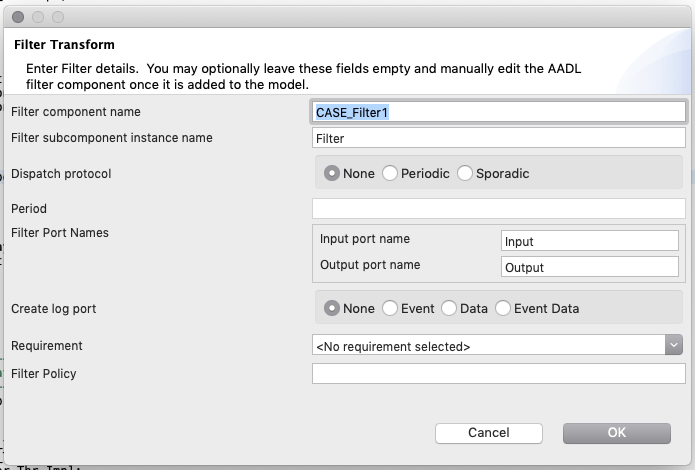
\includegraphics[scale=0.3]{dialogue.png}
%%     \end{tabular}
%%   \end{center}
%%   \caption{BriefCASE dialogue for filter transformation.}
%%   \label{fig:dialogue}
%% \end{figure}


Generally, AGREE contracts do not describe the computation that a
component performs. This is entirely by design: AGREE is intended to
reason about component behavior solely at the specification
level. However, the syntax of AGREE provides enough expressiveness to
support the notion of a \emph{code contract}: a contract from which an
implementation can be extracted. First we must discuss a class of
guarantees---\emph{output guarantees}---which determine the values on
all output ports of a component.

\begin{definition}[Output guarantee]
An \emph{output guarantee} is a stylized guarantee that fully
specifies the data written to an output port. There are three
possibilities according to whether the output port $p$ is
a \konst{data} port, an \konst{event} port, or an \konst{event data}
port:
\[
\begin{array}{ll}
\konst{data}: &  p = \mathit{e} \\
\konst{event}: &  \konst{event} (p) = \mathit{b} \\
\konst{event data}: & \itelse{b}{\konst{event} (p) \land p = e}{\neg \konst{event}(p)} \\
\end{array}
\]
\end{definition}

Informally, a code contract treats its \konst{eq} ``statements'' as
defining a list of assignments to state variables, and its output
guarantees as directives for producing output.

\begin{definition}[Code contract] A
  leaf component of the form $(I,O,A,P,\emptyset)$ is a
  \emph{code contract} if $\mathit{Eqs} \cup G \subseteq P$, where
\[\mathit{Eqs} = \set{v_1 = e_1, \cdots , v_n = e_n} \] is a non-empty set
of \konst{eq} statements and $G$ is the set of output guarantees, one for
each element of $O$. In the interpretation as code, the order of
elements of $\mathit{Eqs}$ is important, and is simply taken to be the
occurrence order of the \konst{eq} statements in the syntax. Thus we
will work with the
\emph{list} of equations $\mathit{Eqs} = [v_1 = e_1; \cdots ; v_n = e_n]$.
\end{definition}


The semantics of Section \ref{agree-semantics} supports a formal
connection between the original contract---and verification results of
the AGREE model checker being run on it---and code generated from
specifications of leaf level cyber-components. It also provides the
root meaning at the base of a chain of translation steps moving from
an AGREE contract to a CakeML executables.

The first step in the chain maps the contract to a code-focused
representation. Assume given a code contract
$(I,O,A,\mathit{Eqs} \cup G \cup P,\emptyset)$, environment $E$, and
time $t$. The \emph{evaluation} of $\mathit{Eqs}$ followed by the
evaluation of $G$ results in a new environment $E'$ where the stream
values for state variables and outputs have been computed for time
$t$. The step from $E$ to $E'$ is one full cycle in the repeated
evaluation of the component.

\begin{definition}[Evaluation]
We overload existing notation and write the evaluation of
$\mathit{Eqs}$ and then $G$ in environment $E$ at time $t$ as
$\sem{\mathit{Eqs}\cdot G}^E_t$. The evaluation of $v = e \in {\Eqs}$
is an environment transformation
\[
 \sem{v = e}^E_t = E[v(t) \mapsto\sem{e}^E_t] \ .
\]
modifying $E$ so that stream $v$ has value $\sem{e}^E_t$ at time $t$.
The list {\Eqs} is evaluated by folding the transformation left-to-right
through it. The transformation is similarly applied to the list of output
guarantees $G$, computing the values on output ports. The details are
omitted, being a bit messy because of the different kinds of output
ports available.
\end{definition}


\begin{definition}[Code contract correctness]
Assume code contract $(I,O,A,\mathit{Eqs} \cup G \cup P,\emptyset)$.
The contract is \emph{correct}, if for all $E$ and $t$, whenever the
assumptions (historically) hold in $E$ and evaluation steps from $E$
to $E'$, then the guarantees hold in $E'$:
\[
\sem{\konst{Hist}(A)}^E_t \land E' = \sem{\mathit{Eqs} \cdot G}^E_t \imp \sem{P}^{E'}_t
\]
\end{definition}
\footnote
{KLS: At this point we would like to assert that the AGREE ``consistency
 check'' for a contract implies code contract correctness.}

How does this notion of correctness integrate with the verification
conditions addressed by model checking? In \emph{contract
correctness}, the model checker is proving the following property
\[
\konst{Hist}(A) \imp P
\]
and in \emph{code contract correctness} we essentially prove a Hoare
triple of the form
\[
\set{\konst{Hist}(A)}\; (\mathit{Eqs} \cdot G) \; \set{P}
\]
This accords with intuition, namely that AGREE is a kind of
`program-free program logic'; by pulling out a program $(\mathit{Eqs}
\cdot G)$ from a code contract we find ourselves in the tepid
bathwater of imperative program verification. For example, at this
point one could apply a verification condition generator to help break
down the proof obligation. In order to use the code contract result in
system contract verifcation conditions, one has to show that the code
contract result implies the system verification condtion.

\subsubsection*{Wellformedness}
The evaluation semantics given above is based on the stream
computation model, where values arbitrarily `deep in the past' can be
accessed in computations by use of $\konst{pre}(-)$. However, the
conventional program languages we target do not support such a
view. We are currently examining transformations that compile such
deep temporal accesses away by introducing intermediate
variables. Avoiding discussion of the algorithm, we focus on the
notion of \emph{wellformed} equations that needs to hold. The guiding
intuition is that an \emph{implementable} {\Eqs} can allow access at
most one step in the past, and accesses of a past value for a variable
are only possible until the variable is updated. In lieu of a formal
definition, we give a few examples.

\begin{definition}[Wellformedness]

\end{definition}

\subsection{Code contracts for the hardened system}

\newsavebox{\flt}
\begin{lrbox}{\flt}
  \begin{lstlisting}[style=agree,numbers=left]
    -- start user definitions
    eq policy : bool =
      WELL_FORMED_AUTOMATION_RESPONSE(Input);
    -- stop user definitions

    guarantee "Filter output is well-formed" :
      if event(Input) and policy then
        event(Output) and Output = Input
      else
        not event(Output);
  \end{lstlisting}
\end{lrbox}

\newsavebox{\mntr}
\begin{lrbox}{\mntr}
  \begin{lstlisting}[style=agree,numbers=left]
    const is_latched : bool = true;

    -- start user definitions
    assume "One automation request in flight at a time" : *\label{line:mon-assume}*
      true -> (req => pre(Historically(not req) or Since(not req, rsp)));

    const MAX_LATENCY : int = 1; *\label{line:mon-const}*

    eq rsp : bool = event(Response);
    eq req : bool = event(Request);

    eq isPending : bool = Since(not rsp, req and not rsp);*\label{line:mon-pending}*
    eq latency : int = 0 -> (if req then 0 else pre(latency) + 1);*\label{line:mon-latency}*

    eq policy : bool = (rsp => req) ->
                         (    (isPending => latency < MAX_LATENCY)
                          and (rsp => (req or pre(isPending))));
    *\label{line:mon-policy}*
    -- stop user definitions

    eq alert : bool = (not policy) -> *\label{line:mon-alert}*
                        ((is_latched and pre(alert)) or not policy);

    guarantee "Alert port tracks alert variable" :
      event(Alert) = alert;
    guarantee "Output if not alerted" :
      if (not(alert) and rsp) then
          event(Output) and (Output = Response)
      else
          not (event(Output));
  \end{lstlisting}
\end{lrbox}

\begin{figure}
  \begin{center}
    \begin{tabular}{c}
      \scalebox{0.62}{\usebox{\flt}} \\
    \end{tabular}
  \end{center}
  \caption{Code contract specification for high-assurance filter.}
  \label{fig:filter}
\end{figure}

\begin{figure}
  \begin{center}
    \begin{tabular}{c}
    \scalebox{0.62}{\usebox{\mntr}} \\
    \end{tabular}
  \end{center}
  \caption{Code contract specification for high-assurance monitor.}
  \label{fig:monitor}
\end{figure}


As previously discussed, transformations carried out in the BriefCASE
interface have created a cyber-hardened system, protecting against
malicious AI behavior, by inserting a high-assurance filter and
monitor between the AI and the WM (see \figref{fig:hardened}). The
filter protects the WM from malformed data and the monitor protects
the WM from (possibly malicious) spontaneous or delayed responses.
These components were added, one at a time, by
\begin{enumerate}
  \item selecting the connection in the model where the
    component is to appear,
  \item choosing the appropriate transformation, and
  \item specifying the relevant filtering or monitoring \emph{policy} (behavior).
\end{enumerate}

%% The system designer provides configuration parameters for the
%% transformation in a dialogue box.  The dialogue box for adding a
%% filter is shown in \figref{fig:dialogue}.  All high-assurance
%% components rely on a \emph{policy} to define behavior as seen in the
%% last field of the dialogue box.  A filter policy defines well-formed
%% data while a monitor policy defines an invariant over inputs and
%% outputs.  These policies can be stated directly in the wizard, or they
%% can be left blank and added later to the AGREE contract generated by
%% the transformation.

BriefCASE creates all the needed AADL for the new high-assurance
component, and its connections in the system implementation, as part
of the transformation.  It also creates a default AGREE specification
that defines everything about the component behavior, leaving only the
component behavior (policy) to be specified.


Code contracts for the filter and monitor are shown in
\figref{fig:filter} and \figref{fig:monitor}.\footnote{KLS: do we discuss wellformedness anywhere?} In general, the
\konst{eq}-statements of a code contract keep track of
state and provide data values from which to compute values to place on
the outputs.

\subsubsection{Monitor specification}
BriefCASE generates everything but the
\konst{eq}-statements in \linesref{line:mon-assume}{line:mon-policy} of
\figref{fig:monitor}.  As with the filter, the guarantees
completely define the output, as required for synthesis, in terms of
the policy and the alert.  The
\texttt{alert} variable defined on \lineref{line:mon-alert} depends
not just on the policy but also on configuration details supplied when
the component is specified.  At configuration
time, \texttt{is\_latched} has been set to \konst{true}, thus making
the alert persistent, meaning that once the alert is raised, it is
always raised; otherwise, it is the complement of the policy value in
the current step.

The monitor policy is defined by marking when a request is not
satisfied, \texttt{isPending} on \lineref{line:mon-pending}, and
counting the number of steps between requests, \texttt{latency} on
\lineref{line:mon-latency}.  The \texttt{isPending} variable is true
whenever there is a request that does not coincide with a
response--\emph{not response since request and not response}.  The
\texttt{latency} variable starts at zero, resets on every request, and
otherwise increments by one.

The latency bound for the monitor is defined by the constant
\texttt{MAX\_LATENCY} on \lineref{line:mon-const}.  Here the constant
is set to one to be consistent with the system specification from the
previous section.  At time 0 the policy is trivial: a response
requires an accompanying request.  After time 0, if a request is
pending in the current time step, then the latency must still be under
the bound, and if there is a response, then it closes a request now or
a pending request from earlier in time.

The policy definition only works if there is never more than one
outstanding request at a time; otherwise, the latency counter resets
incorrectly.  That requirement is encoded in the assumption on
\lineref{line:mon-assume} and is the same assumption used for the
system input.  The policy can be written without needing the
assumption, but it is much simpler to write with the assumption.

As shown in \figref{fig:hardened-certificate}, the cyber-hardened
system passes AGREE verification.  That means that the high-assurance
components protect the WM from the untrusted AI generating malformed
data, spontaneous responses, or delayed responses.  Synthesis must
generate precise implementations of the high-assurance component
specifications for the AGREE verification result to apply to the
deployed system.  Precise in this context means that the
implementations match the input to output relations defined in the
specifications.


\ifREVISIONS
\subsection{Revisions}
\begin{compactitem}
  \item \sout{Add in intuitive definition or AGREE leaf-component semantics}
  \item State well-formed theorem
  \item State correctness theorem or any key theorems to the synthesis proof
\end{compactitem}
\fi

\section{Testing Specifications with AGREE}
\label{sec:testing}
Before discussing the final steps in synthesis, we take a moment to discuss how code-contracts, and any AGREE specification in general, can be traditionally tested to build assurance.
Writing and proving properties about AGREE specifications is hard not just because it is a formal process but  because it reasons about constraints that define the entire input space for a component, and the entire output space, at once.
The case studies showed that engineers, and formal method practitioners, make mistakes writing these specifications especially if the computation or temporal reasoning is complex.

Four common mistakes in specifications have been observed: contradictions, vacuity, under-specification, and missed corner cases.
Contradictions arise from inconsistent contracts that state conflicting constraints in any given moment invalidating the verification results.
Vacuity is a common pitfall with implication when the left hand side is always false making the implication true. 
Under-specification is very challenging because verification is not able to prove anything (or it can prove everything in the case of existential properties) so nothing is actually known after verification except that the system is under-specified. 
Missed corner cases is a common problem to all disciplines.
It is especially hard here because there is no direct way to provide test input and check test output.

AGREE already detects, and reports, contradicting and inconsistent contracts, but it does not check for vacuity and under-specification.
The tempting approach to check these issues is to use the synthesize path and then apply traditional testing.
Such an approach adds extra steps that are not needed as it is possible to bridge the formal model in AGREE with its proof system to traditional reasoning with test.

Unit tests are created in AGREE by writing a system specification that assumes the test input and then guarantees the test output.
The system is then implemented with the component under test and its specification.
The AGREE analysis then proves if the component guarantees, given the test inputs, are strong enough to prove the guaranteed test outputs.
Here the system assumptions strengthen the component assumptions to a single input, and the system guarantees weaken, or leave unchanged, the component output for that test input, depending on the goal of the test.
AGREE proves the component implements the test, and the Liskov substitution principle holds.

\newsavebox{\tst}
\begin{lrbox}{\tst}
  \begin{lstlisting}[style=agree,numbers=left]
    process should_notAlertAndOutput_when_responseOneStepAfterRequest
      ... -- Omitted AADL features
      annex agree {**
        eq index : int = prev(index + 1, 0); *\label{line:tst-index}*
        
        assume "One Response one step after Request" : *\label{line:tst-assume-1}*
                ((index = 0) => not event(Response))
            and ((index = 1) => event(Response))
            and ((index >= 2) => not event(Response));
        assume "One Request" : *\label{line:tst-assume-2}*
            (event(Request) = true) ->
            (event(Request) = false);
        
        guarantee "Not Alert" : *\label{line:tst-guarantee-1}*
            not event(Alert);
        guarantee *\label{line:tst-guarantee-2}*
          "Output one step after Request at same time as Response" :
                ((index = 0) => not event(Output))
            and ((index = 1) => (event(Output) and Output = Response))
            and ((index >= 2) => not event(Output));
      **};
    end should_notAlertAndOutput_when_responseOneStepAfterRequest;
    
    process Implementation *\label{line:tst-imp-start}*
      should_notAlertAndOutput_when_responseOneStepAfterRequest.test
      subcomponents
        Monitor: thread CASE_Monitor_Thr.Impl; *\label{line:tst-imp-comp}*
      connections
        c00: port Response -> Monitor.Response;
        c01: port Request -> Monitor.Request;
        c02: port Monitor.Alert -> Alert;
        c03: port Monitor.Output -> Output;
    end should_notAlertAndOutput_when_responseOneStepAfterRequest.test; *\label{line:tst-imp-end}*
  \end{lstlisting}
\end{lrbox}

\begin{figure}
  \begin{center}
    \begin{tabular}{c}
    \scalebox{0.62}{\usebox{\tst}} \\
    \end{tabular}
  \end{center}
  \caption{AGREE Unit test for high-assurance monitor.}
  \label{fig:test}
\end{figure}

\figref{fig:test} is a unit test for the high-assurance monitor in \figref{fig:hardened}.
The test checks if the monitor output coincides with the response that comes one step after the request.
It also checks that the alarm does not fire.
\lineref{line:tst-index} creates an index to use to create the test input.
\lineref{line:tst-assume-1} defines when the response appears relative to the index.
\lineref{line:tst-assume-2} defines the request behavior.
\linesref{line:tst-guarantee-1}{line:tst-guarantee-2} define the expected test output.
The test additionally proves that nothing happens after the initial test input and output (e.g., no more input is provided and no more output is generated).
AGREE proves the test correct.
\linesref{line:tst-imp-start}{line:tst-imp-end} implement the system using the component (\lineref{line:tst-imp-comp})

This AGREE test method is effective for detecting vacuity, under-specified behavior, and missed corner cases.
It enables designers to iteratively develop specifications inside the MBE framework using AGREE, and it builds assurance that the specification reflects the desired behavior with black-box, white-box, and other test coverage metrics.
These same tests can be synthesized to the backend implementation for traditional testing.

%% \section{Synthesis from code contracts}
%% \label{sec:semantics}
%% In this section we give an overview of the AGREE semantics, a
machine-checked formal definition of the meaning of AGREE expressions,
formulas, and contracts. The semantics supports a formal connection
between the results of the AGREE model checker and code generated from
specifications of leaf level cyber-components. It also provides the root
meaning at the base of a chain of translation steps moving from AGREE
specifications to CakeML executables.

Code generation is a multi-step transformation that starts with a code
contract and ends with an executable. The first step maps the contract
to a code-focused representation. Assume given code contract
$(I,O,A,\mathit{Eqs} \cup G \cup P)$, environment $E$, and time
$t$. The evaluation of $\mathit{Eqs}$ followed by the evaluation of
$G$ results in a new environment $E'$ where the stream values for
state variables and outputs have been computed for time $t$. The step
from $E$ to $E'$ is one full cycle in the repeated evaluation of the
component.

\begin{definition}[Evaluation]
We overload existing notation and write the evaluation of
$\mathit{Eqs}$ and then $G$ in environment $E$ at time $t$ as
$\sem{\mathit{Eqs}\cdot G}^E_t$. Each $v = e \in {\Eqs}$ is treated as
an environment transformation
\[
 \sem{v = e}^E_t = E[v(t) \mapsto\sem{e}^E_t] \ .
\]
modifying $E$ so that stream $v$ has value $\sem{e}^E_t$ at time $t$.
{\Eqs} is evaluated by folding the transformation left-to-right
through it. The transformation is also applied to the list of output
guarantees $G$, computing the values on output ports. The details are
omitted, being a bit messy because of the different kinds of output
ports available.
\end{definition}


\begin{definition}[Code contract correctness]
Assume given code contract $(I,O,A,\mathit{Eqs} \cup G \cup P)$ and
environment $E$.  The contract is \emph{correct}, if for all $t$,
whenever the assumptions (historically) hold in $E$ and evaluation
steps from $E$ to $E'$, then the guarantees hold in $E'$:
\[
\sem{\konst{Hist}(A)}^E_t \land E' = \sem{\mathit{Eqs} \cdot G}^E_t \imp \sem{P}^{E'}_t
\]
\end{definition}
\footnote
{KLS: At this point we would like to assert that the AGREE ``consistency
 check'' for a contract implies code contract correctness.}

The evaluation semantics given above is based on the stream
computation model, where values `deep in the past' can be accessed in
computations. However, the conventional program languages we wish to
target do not support such a view. Thus code generation is only
defined for a class of \emph{well formed} equations.

\begin{definition}[Wellformedness]

\end{definition}

\subsubsection{Example}




\section{Synthesis to CakeML}
\label{sec:synthesis}
Synthesis maps from model and specifications to code. The synthesis
algorithm traverses the system architecture looking for occurrences of
filter and monitor specifications;  for each such occurrence it
generates a CakeML program. In the following, we examine both filter
and monitor synthesis. The latter is typically much more involved, and
we will therefore devote more attention to it.

\subsection{Filter Generation}

A filter is intended to be very simple; it is expected to have one
input port and one output; messages on the input that the filter
policy admits pass unchanged to the output port; all others are
dropped (not passed on). We have explored in our work two kinds of
filter. In the first, a relatively shallow scan of the input buffer
can enforce the policy. For example, we have used the expressive power
of Contiguity Types \cite{contiguity-types} to enforce
\emph{lightweight} bounds constraints on GPS coordinates in UxAS
messages. On the other hand, the second kind of filter will parse the
input buffer into a data structure specified in AGREE and apply an
user-defined \emph{well-formedness} property, also specified in AGREE,
to the data. This allows arbitrarily complex well-formedness checking.

The decision of a filter is made and performed within one thread
invocation. Thus, in its given time slice, the filter does the following:

\begin{enumerate}

\item checks to see if there is any input available; if there is none
then it yields control; otherwise,

\item the input is read (and parsed if need be),

\item the wellformedness predicate is evaluated,

\item if the predicate returns \konst{true} then the input buffer
 is copied to the output; otherwise no action is taken, and

\item the filter yields control
\end{enumerate}

\begin{remark}[Partiality]

The role of partiality should be emphasized: steps 2 and 3 can fail;
the data might not be parseable or the wellformedness computation
could be badly written and fail at run time. In such cases, the filter
should recover and yield control without passing the input onwards. In
these cases, the filter is behaving as it should, but there are also
cases in which a correctly specified filter would not meet its
specification at runtime. This situation arises when the
filter \emph{ought} to accept a message, but lack of resources result
in the filter failing to do so. Examples of this would be, for
example, if the parse of a message needed more space than allocated;
another example would be if the timeslice provided by the scheduler is
too small for the wellformedness computation to finish.

\end{remark}


{\emph{Need some discussion of filters and their step-wise properties
  in relation to their infinitary properties. Reference to Johannes'
  work.}

\newsavebox{\contig}
\begin{lrbox}{\contig}
\begin{lstlisting}[style=myML]
  Waypoint =
    {Latitude  : f64
     Longitude : f64
     Altitude  : f32
     Check     : Assert
      (~90.0 <= Latitude and Latitude <= 90.0 and
       ~180.0 <= Longitude and Longitude <= 180.0 and
       1000.0 <= Altitude and Altitude <= 15000.0)}

  AutomationResponse =
    {TaskID : i64
     Length : u8
     Waypoints : Waypoint [3]}
\end{lstlisting}
\end{lrbox}

\begin{figure}
  \begin{center}
    \begin{tabular}{c}
      \scalebox{0.60}{\usebox{\contig}}
    \end{tabular}
  \end{center}
  \caption{Contiguity type specification for filter.}
  \label{fig:filter-contig}
\end{figure}


\newsavebox{\cml}
\begin{lrbox}{\cml}
\begin{lstlisting}[style=myML]
fun filter_step () =
 let val () = Utils.clear_buf buffer
     val () = API.callFFI "get_input" "" buffer
 in
    if WELL_FORMED_AUTOMATION_RESPONSE buffer
    then
      API.callFFI "put_output" buffer Utils.emptybuf
    else print"Filter rejects message.\n"
end
\end{lstlisting}
\end{lrbox}

\begin{figure}
  \begin{center}
    \begin{tabular}{c}
      \scalebox{0.60}{\usebox{\cml}}
    \end{tabular}
  \end{center}
  \caption{Synthesized CakeML for the filter.}
  \label{fig:filter-cakeml}
\end{figure}

The contiguity type specification for the filter is shown in
\figref{fig:filter-contig}. The synthesized CakeML code for the filter is shown in
\figref{fig:filter-cakeml}. The code is called at dispatch by the
scheduler. The \texttt{API.callFFI} is the link to the communication
fabric to capture input and provide output. The body of the function
restates the filter contract to make the appropriate assignments in a
way that matches the truth value of the predicate in the filter
guarantee.  The auto-generated AGREE specification raises an alert
output when the relation is violated.

% A \emph{system} is a collection of \emph{components}, \emph{connections}
% between components, a \emph{scheduler} to order execution, and a
% \emph{system environment} for primary inputs.

\subsection{Monitor Generation}

Monitors, since they are intended to track and analyze the externally
visible behavior of system components through time, require more
computational features than filters. In particular, our conception of
a monitor is a predicate on its input (and output) streams, being able
to access the value of a stream at any earlier point in time, if
necessary. Thus monitors commonly use state to keep track of earlier
values, unlike filters which are stateless. This reasoning leads us to
specify the computation for a monitor component by a step function of
the following form:
\[
\konst{stepFn} : \mathit{input} \times \mathit{stateVars} \to \mathit{stateVars} \times \mathit{output}
\]
Thus, in its given timeslice, a monitor evaluates the \konst{stepFn} on its inputs and the current values of the state variables. In detail, it takes the following steps:

\begin{enumerate}

\item each available input is parsed into data of the type specified
by the port type;

\item the stateful variables in $\mathit{stateVars}$  are evaluated in dependency order.

\item values of outputs are computed

\item outputs are written and the new state is written

\item control is yielded
\end{enumerate}

Our earlier remarks on partiality apply here too, of course.


The scheduler \emph{activates} components in some order.It is an
obligation on the system that the scheduler follows some sensible
partial order of component activation and allows each component
sufficient time for its computation.  Activating a monitor component
takes the form of the following pseudo-code:
\[
\begin{array}{ll}
 \mathit{(i_1,\ldots)} & = \konst{readInputs}(); \\
 (v_1,\ldots) & = \konst{readState}() ; \\
 ({v_1}',\ldots), ({o_1}',\ldots) & = \konst{stepFn} ((i_1,\ldots),(v_1,\ldots)) ; \\
 \multicolumn{2}{l}{\konst{writeState}({v_1}',\ldots);} \\
 \multicolumn{2}{l}{\konst{writeOutputs}({o_1}'\ldots);} \\
\end{array}
\]

\paragraph{Initialization}
A monitor may need to accumulate a certain minimum number of
observations before being able to make a meaningful assessment of
behavior. Until that threshold is attained, the monitor is essentially
in a kind of \emph{initialization} phase. In order for correct code to
be generated, monitor specifications need to spell out the values of
output ports when in an initialization phase. For example, suppose a
monitor does some kind of differential assessment of inputs at
adjacent timeslices, alerting when (say) the measured location of a
UAV at times $t$ and $t+1$ is such that the distance between the two
locations is unusually large. Such a monitor needs two measurements
before making its first judgement, but at the time of its first
output, only one measurement will have been made. The specification
for must explicitly state what the correct first output is.


\ifREVISIONS
\subsection{Revisions}
\begin{compactitem}
  \item State theorem relating the step function to the meaning of the leaf-node semantics
\end{compactitem}
\fi

\section{Case studies}
\label{sec:case-study}
In this section, we apply the BriefCASE tool to the development of a UAV surveillance system in which a UAV receives commands from a ground station to conduct surveillance along a geographical feature such as a river. The on-board mission computer then generates a flight plan consisting of a series of waypoints that the UAV must traverse to complete its mission. The UAV is also given a set of \textit{keep-in} and \textit{keep-out} zones that may constrain its flight path.

We have modeled the system architecture of the UAV in AADL.  It includes a Mission Computer for communicating with the ground station and generating flight plans, and a Flight Control Computer for UAV navigation.  The Mission Computer architecture model includes hardware components such as a processor, memory, and communication devices, as well as software.
%
The initial software architecture model (shown in Figure~\ref{fig:sw-initial}) contains drivers for communication with the Ground Station and Flight Control Computer, a Waypoint Manager component that provides flight plan coordinates to the Flight Control Computer, and the Flight Planner.  The Flight Planner is the open-source UxAS software developed by AFRL~\cite{uxas}. 

For this application, UxAS accepts three types of messages.  The \textit{Operating Region} message defines where the UAV can and cannot fly.  The \textit{Line Search Task} message contains a series of waypoints that the UAV should traverse.  The waypoints typically lie along some geographical feature of interest, such as a river or railway.  Note that the UAV may not be able to directly traverse the Line Search Task waypoints due to no-fly zone constraints specified in the Operating Region message.  Anytime after receiving the Operating Region and Line Search Task messages, a ground station can transmit an \textit{Automation Request} message, which instructs UxAS to generate a flight plan that satisfies these constraints.  UxAS passes the flight plan in an \textit{Automation Response} message to the Waypoint Manager.  Because the Flight Control Computer can only process a small number of waypoints at a time, the Waypoint Manager parcels a small number of waypoints corresponding to the current UAV position, and sends them to the Flight Control Computer over a serial connection via the UART Driver.

\begin{figure}[h]
	\centering
	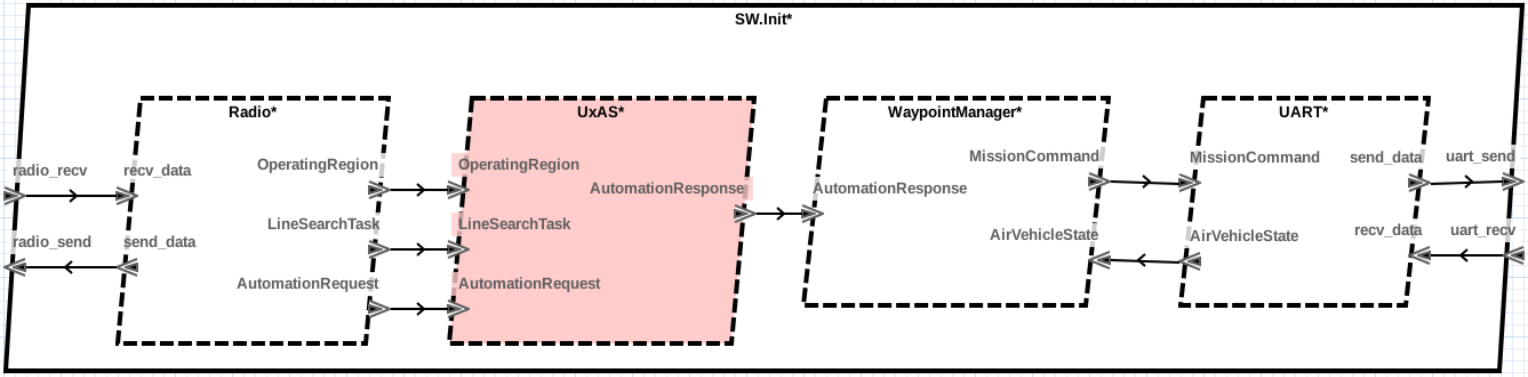
\includegraphics[width=1\columnwidth]{figs/sw-initial.png}
	\caption{Initial software architecture.} 
	\label{fig:sw-initial} 
\end{figure}

Within the software model, we have formalized some of the high-level requirements as assume-guarantee contracts.  We perform a formal analysis using the AGREE tool (which is integrated with the BriefCASE environment) to verify that the model satisfies the contracts.  For the initial version of our design, the verification passes.
%
Although we are satisfied with the results of the formal verification using AGREE, we have not yet analyzed the design for cyber-vulnerabilities.  
In BriefCASE, we analyze the model using one (or more) of the integrated cybersecurity analysis tools.  The tools generate a list of new requirements corresponding to cyber vulnerabilities found in the design.  To satisfy these requirements we need to mitigate the vulnerabilities discovered by the analysis by modifying the design.
%
For example, because we annotated the open-source UxAS component as \texttt{uncontrolled} (colored red in Figure~\ref{fig:sw-initial}), the cyber analysis tools generate requirements for ensuring unverified or malicious code (that could potentially be included in the component) will not impact other processes. 

In total, seven cyber requirements are generated and imported into our model.  These include four \textit{well-formedness} requirements, two requirements for \textit{monitoring} the behavior of the open-source UxAS component, and an \textit{attestation} requirement for ensuring the Ground Station software has not been tampered with.  Requirements are imported into the model as goals in a Resolute assurance case.  Because we can run Resolute at any time during development, we can easily determine for a given snapshot of the model which requirements are not yet supported by evidence.

The intent of the \textit{well-formedness} requirements is to prevent malformed messages from causing a buffer overrun or code injection attack.  In the UAV design, such messages are most likely to originate from a remote source or the uncontrolled UxAS component.  By placing filters on the connections upstream of mission-critical components, such attacks could be mitigated.  The Filter transform is therefore applied for each well-formedness requirement, inserting filter components on the incoming and outgoing UxAS connections.  

The filter behavior for each component is specified in AGREE.  Not only does this enable formal verification within the modeling environment, but it also provides a means for synthesizing the component implementation in a provably correct manner using the SPLAT tool.  Because SPLAT is integrated with BriefCASE, the proof it emits when synthesizing component code is used as evidence in the Resolute goal for the corresponding mitigation.  When Resolute evaluates whether such a goal is supported by evidence, it checks for the existence of the synthesis proof in addition to verifying the architecture is correct.  

The AGREE filter policies for the four UxAS connections are similar, and check that record values contained in the messages are within appropriate ranges.  For example, the Automation Response message filter, which drops message containing malformed flight plans, is defined as shown in Figure~\ref{fig:automation-response-filter}.  Although Latitude, Longitude and Altitude are defined as 64-bit \textit{reals}, the filter ensures only messages containing waypoint values between [-90,9], [-180,180], and [0,15000], respectively. 

\begin{figure}[h]
	\centering
	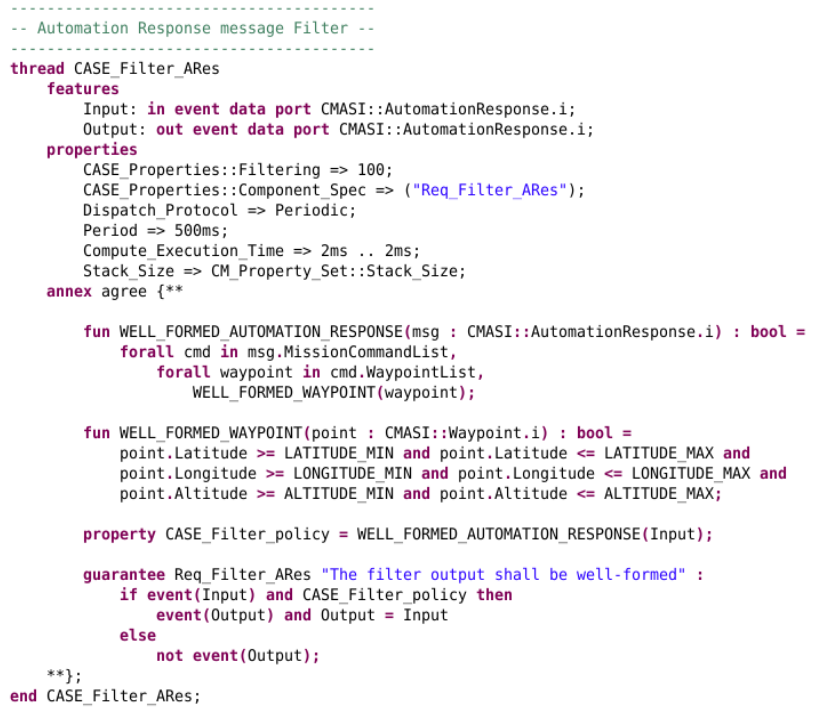
\includegraphics[width=1\columnwidth]{figs/automation-response-filter.png}
	\caption{Automation Response Filter specification.} 
	\label{fig:automation-response-filter} 
\end{figure}

In addition to monitoring the UxAS output for malformed messages, we must also monitor for suspicious behavior.  This requires adding components for detecting that UxAS has crashed, as well as monitoring the correctness of the flight plans it produces.  The Monitor transform is applied for this class of mitigation.  In general, monitors observe a channel and compare its contents against a reference signal or constant.  The monitor policy specifies acceptable comparisons, and if violated, the monitor sends out an alert.  A monitor can choose to \textit{gate} the observed signal, in which case it also acts as a special kind of filter and drops the message if the policy is violated.  The \textit{monitoring} requirements drive two transforms.  The first adds a \textit{response} monitor to send an alert if UxAS does not emit a response within a set amount of time from receiving a request.  The second adds a \textit{geofence} monitor to ensure that generated flight plans are compliant with the specified keep-in and keep-out zones.  The Geofence Monitor is a gated monitor; it prevents the observed Automation Response message from reaching the Waypoint Manager. 

Similar to the filters, the monitor policies are specified in AGREE. For example, 
%The Response Monitor specification is shown in Figure~\ref{fig:response-monitor}, and 
the Geofence Monitor specification is shown in Figure\ref{fig:geofence-monitor}. 

% \begin{figure}[h]
% 	\centering
% 	\includegraphics[width=1\columnwidth]{figs/response-monitor.png}
% 	\caption{Response Monitor specification.} 
% 	\label{fig:response-monitor} 
% \end{figure}

\begin{figure}[h]
	\centering
	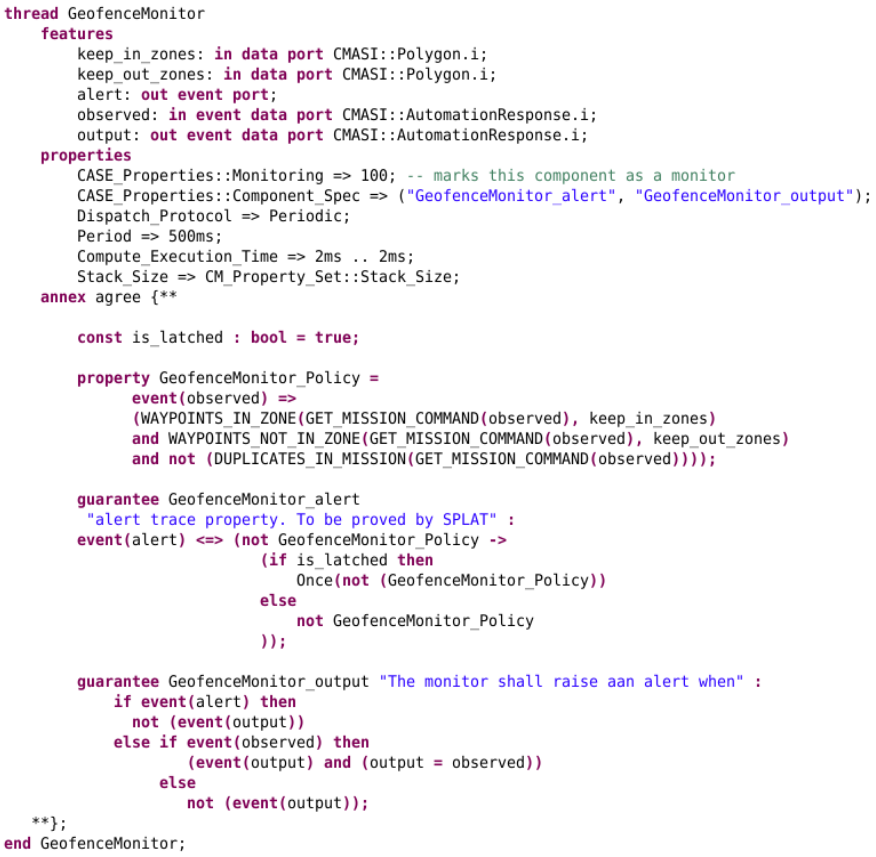
\includegraphics[width=1\columnwidth]{figs/geofence-monitor.png}
	\caption{Geofence Monitor specification.} 
	\label{fig:geofence-monitor} 
\end{figure}

The requirements that have been addressed so far mitigate vulnerabilities related to malformed messages and malicious behavior \textit{on board} the UAV.  But we also want to protect against a compromised Ground Station that could potentially transmit well-formed, but malicious commands. The final cyber-requirement is mitigated by the Attestation transform~\cite{attestation-copland}, which adds two components to the UAV software: an Attestation Manager for evaluating remote systems like the Ground Station, and an Attestation Gate for filtering messages from sources that have not been approved by the Attestation Manager.  The Attestation Manager is implemented in CakeML and automatically inserted into the application code base by BriefCASE.  Because the Attestation Gate acts as a filter, the transform automatically generates its complete AGREE specification.%, as shown in Figure~\ref{fig:attestation}.

% \begin{figure}[h]
% 	\centering
% 	\includegraphics[width=1\columnwidth]{figs/attestation.png}
% 	\caption{Atestation specification.} 
% 	\label{fig:attestation} 
% \end{figure}

After transforming the model to address the cyber requirements, the software architecture now appears as shown in Figure~\ref{fig:hardened-sw}.  The components in green were added to the model by way of an automated BriefCASE transform and are critical for mitigating cyber attacks. 
We formally verify the model with AGREE to show that all of the component contracts are satisfied, including the new contracts introduced during the model transformations.
Because it is imperative that these high-assurance component implementations are correct,
we run the SPLAT tool to produce provably-correct code.  
The synthesized code is output to a directory in the build file system with the location specified for each component in the model.  The corresponding correctness proof is used in our assurance case as additional evidence that the vulnerability has been properly mitigated.

\begin{figure}[h]
	\centering
	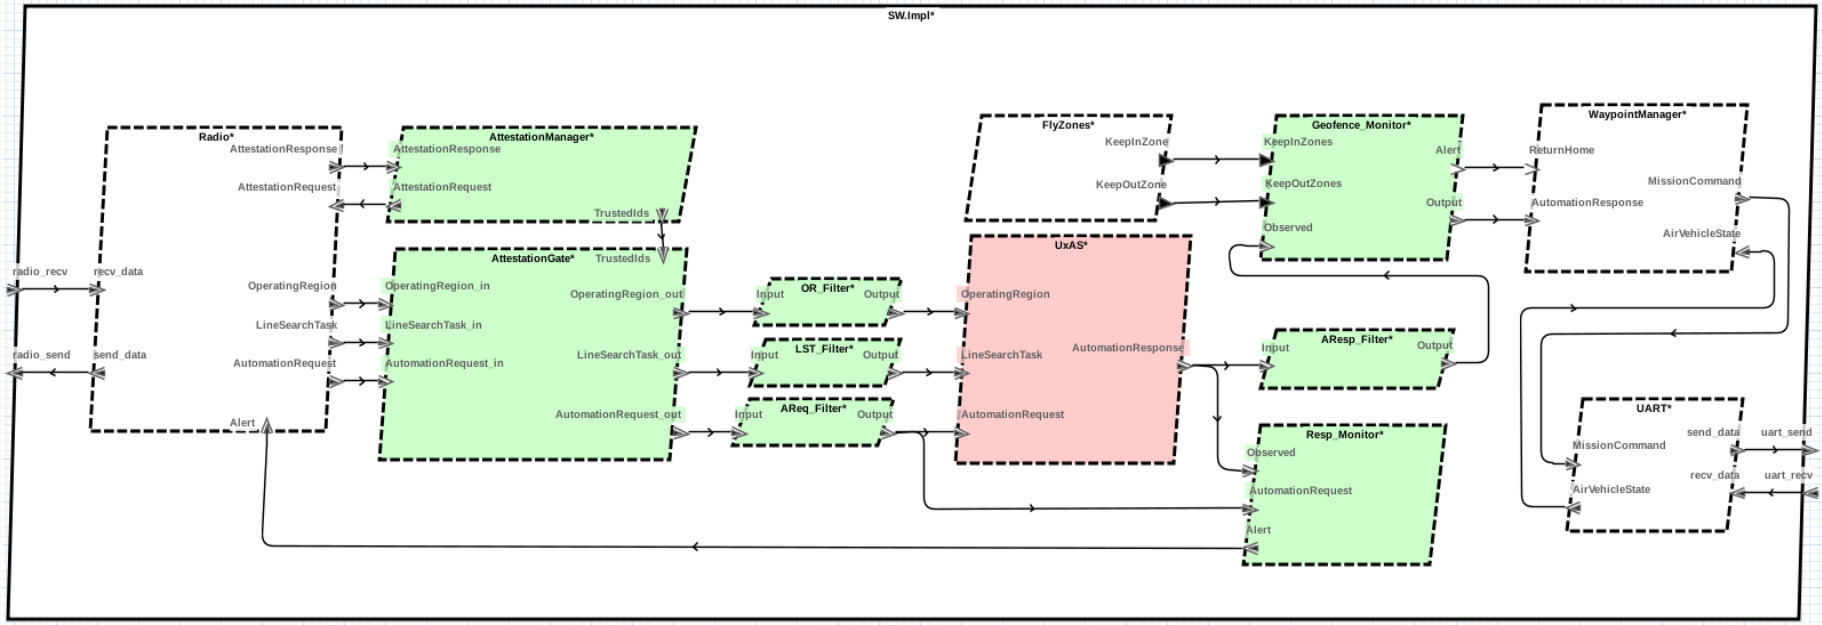
\includegraphics[width=1\columnwidth]{figs/hardened-sw.png}
	\caption{Cyber-resilient software architecture.} 
	\label{fig:hardened-sw} 
\end{figure}

Once we have determined that the model is correct and satisfies its cyber requirements, and the software components in the model have been implemented, either by SPLAT or other means, the system can be built and deployed.  We run the HAMR tool to generate the component stubs and infrastructure code necessary to enable component communication and execution according to a specified schedule.
HAMR translates the AADL system model to code that implements threading infrastructure and inter-component communication and is consistent with the AADL specification computational model.
%
HAMR then compiles the software to execute on seL4~\cite{sel4-2009}, a verified capability-based microkernel (accompanied by formal proof of spatial isolation properties down to the binary level).

The UAV and Ground Station software were deployed on the ODROID XU4 hardware and communicated with each other over Ethernet.  The AMASE flight simulator, representing the Flight Contol Computer was run on a Linux machine and connected to the UAV ODROID via a serial connection.  The UxAS implementation on the UAV was modified by adding malicious code that would prevent it from responding to Automation Requests or produce flight plans that would violate the operating region constraints.  Some of the Line Search Task messages transmitted from the Ground Station contained malformed messages that would modify the UxAS behavior. In addition, we modified the Ground Station to simulate a breach for the attestation test.

We performed an initial set of tests on the un-hardened system (Figure~\ref{fig:sw-initial}) to verify the effectiveness of the malicious code.  The following scenarios were exercised:

\paragraph{Infected Ground Station} In this scenario, one of the UxAS files is modified on the Ground Station. When Ground Station files are modified in such an unauthorized manner, messages sent to the UAV will be rejected by the Attestation Manager.  

\paragraph{Malformed Line Search Task message} In this scenario, the Line Search Task message contains a waypoint with a longitude value outside the permitted range.  Such malformed messages could exploit vulnerabilities in the onboard software.  This vulnerability is mitigated by inserting a well-formedness filter.  The filter prevents the Line Search Task message from reaching UxAS.

\paragraph{UxAS vulnerability exploit} In this scenario, Line Search Tasks with greater than 90 waypoints will trigger a vulnerability that will crash UxAS.   When this occurs, UxAS be prevented from generating an Automation Response.  This vulnerability is mitigated by inserting a Response Monitor, which checks to see that UxAS outputs an Automation Response message shortly after receiving an Automation Request.  For this scenario, we chose for the monitor to output a status message, which would then be received by the Ground Station and an appropriate action taken.

\paragraph{UxAS trojan modifies flight plan} In this scenario, a trojan embedded in UxAS will attempt to cause the UAV to fly into the specified keep-out zone by modifying the mission command waypoints in the Automation Response.  However, the UAV will detect that it is being instructed to fly into a keep-out zone and instead return to Home Base.

We repeated the tests on the hardened system and were able to demonstrate that our mitigations were successful, as indicated by the status messages sent from the high-assurance components, shown in Figure~\ref{fig:mitigation-output}.

\begin{figure}[h]
	\centering
	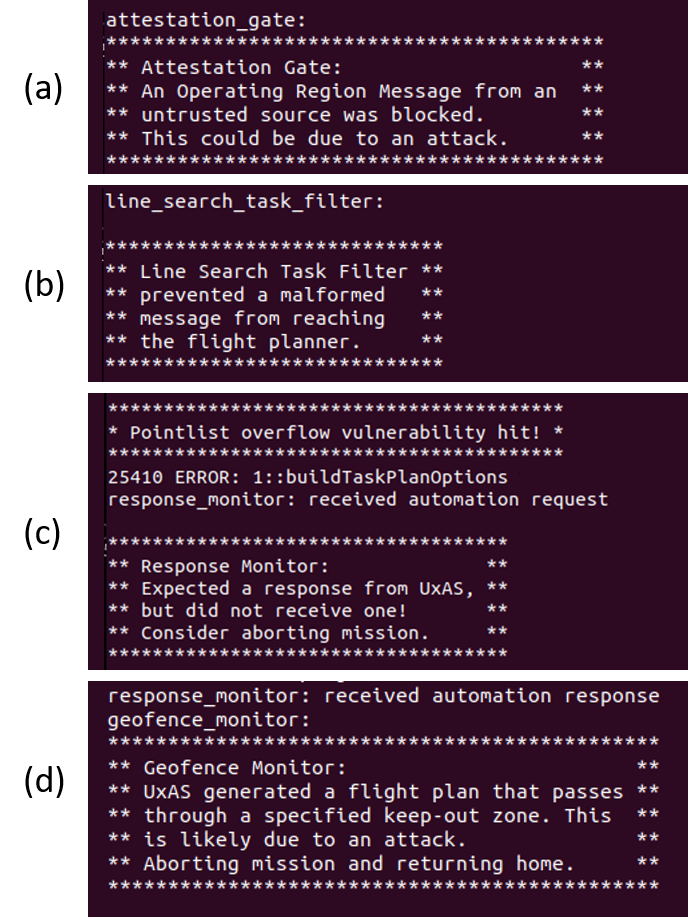
\includegraphics[width=0.8\columnwidth]{figs/mitigation-output.png}
	\caption{Cyber-resilient system response.} 
	\label{fig:mitigation-output} 
\end{figure}



\ifREVISIONS
\subsection{Revisions}
\begin{compactitem}
  \item Possible Outline:
  \begin{compactitem}
    \item Two case studies: phase 2 is the proof on concept on a industrial size problem while phase 3 tests if AGREE is expressive enough for stating complex properties and if designers are able to use it.
    \item Phase 2 write up focusses on the number of components and the relative ease for AGREE to prove out and for SPLAT to synthesize. It notes that the components were relatively simple.
    \item Phase 3 write up focusses on the shear complexity of the components and in particular the gate and the transport monitor. Here it the need for testing is is most obvious. Also obvious is the need to make AGREE more expressive and to separate AGREE into a specification and implementation language as seen in Dafny.
    \item Make the general observation that the transforms on the AADL model to add the components and connections doesn't really save much time when compared against the time it takes to write and test the specifications. The automations is nice, but not where time is saved. Where time is saved is in the assurance case because once a specification is done, it is synthesized and proved correct for ALL inputs and ALL outputs. Not just some. Not code inspections. Not additional test requirements. All that is saved.
  \end{compactitem}
  \item Clarify research questions answered by the case study
  \item Make the figures bigger
  \item Rewrite to focus on synthesized components and the AGREE specifications
  \item Add an interesting monitor from the TA6 model
  \item Discuss what efforts are optimized with the automations versus a fully manual process for creating the components--how does the automated transformation affect actual time for engineers
\end{compactitem}
\fi

\section{Related work}
\label{sec:related-work}
Assume-guarantee reasoning for compositional verification in reactive systems is well-studied \cite{10.1007/978-3-642-28891-3_13, composition1, 10.1145/2658982.2527272, 10.1007/978-3-319-17524-9_7}. Automated proofs of realizability for assume-guarantee reasoning are useful for engineers implementing components in the system \cite{10.1007/978-3-319-17524-9_13, 10.1007/978-3-319-29613-5_7}. Algorithms for actual component synthesis for Lustre models using k-induction or IC3/PDR provide an automated path from the assume-guarantee reasoning to an actual satisfying node implementation \cite{katis2017synthesis, 10.1007/978-3-319-89963-3_10}. These synthesis algorithms generate code in the Lustre modeling language but do not provide a path to a low-level implementation that could be fielded.

Contracts are similar to assume-guarantee reasoning but are targeted to programming languages. Contracts are often more expressive than assume-guarantee reasoning and can not only be stateful but higher-order \cite{10.1145/583852.581484}. As contracts are often written in the target language, synthesis is not a problem for monitoring but comes with significant overhead \cite{10.1007/978-3-642-28869-2_11}. A monitor for a contract can be removed when it can be statically proved that the code preserves the contract under all possible inputs and executions \cite{10.1145/3158139}.

\ifREVISIONS
\subsection{Revisions}
\begin{compactitem}
  \item Add recent work published after 2018
\end{compactitem}
\fi

\section{Conclusion}
\label{sec:conclusion}
Cyber-physical systems must be tolerant to cyber-attacks in the same way they are tolerant to faults. The DARPA CASE program is creating an MBSE environment for designers to integrate cyber-vulnerability analysis and mitigation through the design process to harden systems early in the design process. BriefCASE is the result of that program, and it provides cyber-analysis tools that add cyber requirements to the AGREE specification for the design and architectural transforms with AGREE specifications to satisfy the cyber requirements. BriefCASE is fully integrated into the OSATE AADL modeling environment for ease of use by system engineers.

The filter architectural transformation in BriefCASE prevents malformed data from being propagated downstream to other components while the monitor transformation enforces temporal properties to detect when untrusted components behave maliciously. The components are specified by corresponding auto-generated AGREE contracts that only require the system designer to state the policies to enforce.These can be adapted from the cyber requirements in the system design. The specifications are automatically synthesized to CakeML that can then be compiled to a wide array of backend targets. The synthesis to CakeML is done in a way that preserves the meaning of the specifications.

The BriefCASE tool suite demonstrated in action on a full-scale case study with the UxAS open source UAV AI planning system. The complex system requires several architectural transformations to meet cyber-requirements, and the entire system is synthesized and deployed on the seL4 platform running on ODRIOD using the synthesis tool described here and the BriefCASE HAMR tool to generate the communication fabric. The size and scale of the case study gives some evidence that BriefCASE, with its transformations, scales to the complexity demands often seen in real-world design.

Ongoing work is using BriefCASE on the Collin' Common Avionics Architecture System (CAAS) in the context of a CH47 rotary wing platform \cite{caas}. The filter and monitor transformations are being employed to protect against \emph{Automatic Dependent Surveillance-Broadcast} (ADS-B) spoofing by malicious actors in the airspace. That work is expanding synthesis with uninterpreted functions to support non-linear and transcendental functions. Other ongoing work is mechanizing the synthesis proof in HOL4 and lifting the proof results given for finite streams to infinite streams.

\clearpage
\bibliographystyle{plain}
\bibliography{paper}

% \appendix
% \section{Contiguity Types}
% The formal specification of a component, and the synthesis of that specification, relies on \emph{contiguity types} to define the input and output data (cite contiguity). A contiguity type is a self-describing specification for messages. Its formalism has basis in formal languages. Similar to how a regular expression implies a set of words that form its language, so does a contiguity type specification imply a set of messages for its language where a message is a finite sequence of contiguous bytes (e.g., a string). 

What makes contiguity type specification more expressive than regular expressions is that it is self-describing meaning that the contents of the message itself may determine the rest of the message. An example is the \texttt{AutomationResponse} from the system in the previous section with its contiguity type specification.
{\small
\begin{verbatim}
  {TaskID : i64
   Length : u8
   Waypoints : Waypoint[Length]
  }
\end{verbatim}
}
\noindent The \texttt{Waypoints} array size depends on the value of \texttt{Length} so the actual number of bytes in the message depends on the contents of the message itself. 

The type specifications may also carry meta-information about the contents of the message.
{\small
\begin{verbatim}
  {Latitude : float
   lt-rng : Assert (-90 <= Latitude <= 90) 
   Longitude : float
   lng-rng : Assert (-180 <= Longitute <= 180)
   Altitude : float
   a-rng : Assert (10000 <= Altitude <= 15000)
  }
\end{verbatim}
}
\noindent Here the specification encodes the allowed ranges for each field of the waypoint. These assumptions restrict the resulting language to include only conforming messages and can be checked while constructing a message from a sequence of bytes. The notation $\LangTheta{\tau}$ denotes the language defined by the specification $\tau$ using the environment $\theta$ for expression evaluation.

Every contiguity type specification has a corresponding CakeML \emph{matcher} that when given a message string returns true or false if that message belongs to the language of the specification. If the message does belong to the language, an \emph{environment} is provided to access each part of the message. An environment, $\theta: \lval \mapsto \konst{string}$ binds \emph{L-values} to strings, where an L-value is an expression that can appear on the left hand side of an assignment (e.g., \texttt{AutomationRequest.Waypoints[0].Latitude}). 

The main result of contiguity types is the proof of the relationship between the language of the specification and the synthesized matcher from the specification that is summarized below.
\[
  \konst{match}\; s_1s_2 = \konst{SOME}(\theta, s_2)
  \imp \theta(\tau) \cdot s_2 = s_1s_2 \wedge s_1 \in \LangTheta{\tau}
\]
If there is a match on the substring $s_1$, then reconstituting the string from the resulting environment and concatenating it with $s_2$ yields the original string, and the matched string $s_1$ is in the language of the type specification. 

% \section{System Model and Semantics}
% A \emph{system} is a collection of \emph{components}, \emph{connections} between components, a \emph{scheduler} to order execution, and a \emph{system environment} for primary inputs. The computation for the component in this work is defined entirely by a step function:
\[
\konst{stepFn} : \mathit{inports} \times \mathit{stateVars} \to \mathit{stateVars}
\]
The scheduler \emph{activates} components in some order. Activating a component is defined as follows: 
\[
\begin{array}{ll}
 \mathit{inportVals} & = \konst{readInputs}(); \\
 (v_1,\ldots,v_k) & = \konst{readState}() ; \\
 ({v_1}',\ldots,{v_k}') & = \konst{stepFn} (\mathit{inportVals},\mathit{stateVars}) ; \\
 \multicolumn{2}{l}{\konst{writeState}({v_1}',\ldots,{v_k}');} \\
 \multicolumn{2}{l}{\konst{writeOutputs}({v_1}',\ldots,{v_k}');} \\
\end{array}
\]
It is assumed that the scheduler follows some sensible partial order of component activation and allows each component sufficient time for its computation.


\end{document}
